\documentclass[border=8pt]{standalone}
\usepackage{tikz}
\usepackage{amsmath}
\usetikzlibrary{decorations.pathreplacing,calc}

% Flavour-composition colours: |U_{e j}|^2, |U_{mu j}|^2, |U_{tau j}|^2
\definecolor{cnue}{RGB}{ 38,110,180}
\definecolor{cnumu}{RGB}{198, 62, 55}
\definecolor{cnutau}{RGB}{ 60,150, 95}

% Flavour fractions |U_{alpha j}|^2 below are computed from the NuFIT 5.2
% normal-ordering best fit: sin^2(th12)=0.303, sin^2(th13)=0.02203,
% sin^2(th23)=0.572, delta_CP=197 deg. Each row sums to 1 to 4 decimal places.
%
% \massbar{x}{y}{fe}{fmu}{ftau}{label}
% Draws a flavour-composition bar of total width 3.4cm at (x,y).
\newcommand{\massbar}[6]{%
  \pgfmathsetmacro{\bw}{3.4}%
  \pgfmathsetmacro{\bh}{0.30}%
  \pgfmathsetmacro{\xa}{#1}%
  \pgfmathsetmacro{\xb}{#1+\bw*#3}%
  \pgfmathsetmacro{\xc}{#1+\bw*(#3+#4)}%
  \pgfmathsetmacro{\xd}{#1+\bw}%
  \fill[cnue]   (\xa,#2) rectangle (\xb,#2+\bh);
  \fill[cnumu]  (\xb,#2) rectangle (\xc,#2+\bh);
  \fill[cnutau] (\xc,#2) rectangle (\xd,#2+\bh);
  \draw[black,line width=0.4pt] (\xa,#2) rectangle (\xd,#2+\bh);
  \node[anchor=west,font=\small] at (\xd+0.15,#2+\bh/2) {#6};
}

\begin{document}
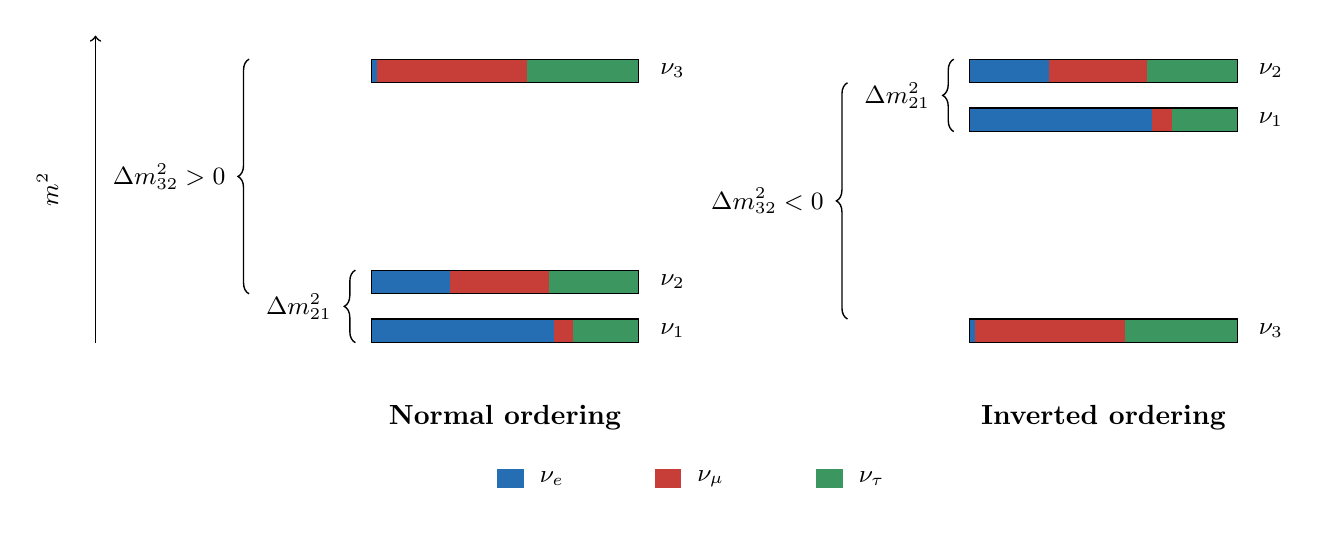
\begin{tikzpicture}[x=1cm,y=1cm]

  % Explicit bounding box, so the crop is deterministic across build environments.
  \path (-4.3,-2.1) rectangle (11.8,4.0);

  % ---------------- Normal ordering (left) ----------------
  \begin{scope}[xshift=0cm]
    % nu_1 and nu_2: solar doublet at the bottom
    \massbar{0}{0.00}{0.6816}{0.0739}{0.2445}{$\nu_{1}$}
    \massbar{0}{0.62}{0.2963}{0.3667}{0.3370}{$\nu_{2}$}
    % nu_3: isolated state above
    \massbar{0}{3.30}{0.0220}{0.5594}{0.4186}{$\nu_{3}$}

    % solar splitting brace (drawn bottom-to-top so it opens towards the bars)
    \draw[decorate,decoration={brace,amplitude=4pt},line width=0.5pt]
      (-0.20,0.00) -- (-0.20,0.92) node[midway,left=5pt,font=\small] {$\Delta m^{2}_{21}$};
    % atmospheric splitting brace
    \draw[decorate,decoration={brace,amplitude=4pt},line width=0.5pt]
      (-1.55,0.62) -- (-1.55,3.60) node[midway,left=5pt,font=\small] {$\Delta m^{2}_{32}>0$};

    \node[font=\bfseries] at (1.7,-0.95) {Normal ordering};
  \end{scope}

  % ---------------- Inverted ordering (right) ----------------
  \begin{scope}[xshift=7.6cm]
    % nu_3: isolated state at the bottom
    \massbar{0}{0.00}{0.0220}{0.5594}{0.4186}{$\nu_{3}$}
    % nu_1 and nu_2: solar doublet above
    \massbar{0}{2.68}{0.6816}{0.0739}{0.2445}{$\nu_{1}$}
    \massbar{0}{3.30}{0.2963}{0.3667}{0.3370}{$\nu_{2}$}

    % solar splitting brace (drawn bottom-to-top so it opens towards the bars)
    \draw[decorate,decoration={brace,amplitude=4pt},line width=0.5pt]
      (-0.20,2.68) -- (-0.20,3.60) node[midway,left=5pt,font=\small] {$\Delta m^{2}_{21}$};
    % atmospheric splitting brace
    \draw[decorate,decoration={brace,amplitude=4pt},line width=0.5pt]
      (-1.55,0.30) -- (-1.55,3.30) node[midway,left=5pt,font=\small] {$\Delta m^{2}_{32}<0$};

    \node[font=\bfseries] at (1.7,-0.95) {Inverted ordering};
  \end{scope}

  % ---------------- Mass-squared axis ----------------
  \draw[->,line width=0.6pt] (-3.5,0.0) -- (-3.5,3.9);
  \node[rotate=90,anchor=south,font=\small] at (-3.85,1.95) {$m^{2}$};

  % ---------------- Legend ----------------
  \begin{scope}[yshift=-1.85cm,xshift=1.6cm]
    \fill[cnue]   (0.00,0) rectangle (0.34,0.24);
    \node[anchor=west,font=\small] at (0.42,0.12) {$\nu_{e}$};
    \fill[cnumu]  (2.00,0) rectangle (2.34,0.24);
    \node[anchor=west,font=\small] at (2.42,0.12) {$\nu_{\mu}$};
    \fill[cnutau] (4.05,0) rectangle (4.39,0.24);
    \node[anchor=west,font=\small] at (4.47,0.12) {$\nu_{\tau}$};
  \end{scope}

\end{tikzpicture}
\end{document}
